\section {Cronograma de actividades}\noindent
En el primer semestre se recopilará información de forma aislada así como integrada con aplicaciones afines al proyecto de investigación.\\
Durante el segundo semestre se construirán los modelos para el almacenamiento en bases de datos.\\
En el tercer semestre se generará la metodología para la obtención del conjunto de palabras para extender la búsqueda y estimar modelos de regresión, y se desarrollará el método para realizar nuevas búsquedas correlacionadas y complementaria a la palabra clave.\\
Finalmente en el cuarto semestre se obtendrán parámetros de estimación para el modelo de regresión lineal utilizando los datos de la búsqueda y se realizarán pruebas de hipótesis. Se construirán elementos gráficos usando distribuciones y rectas de regresión lineal y se comunicarán los resultados.
\begin{figure}[H]\centering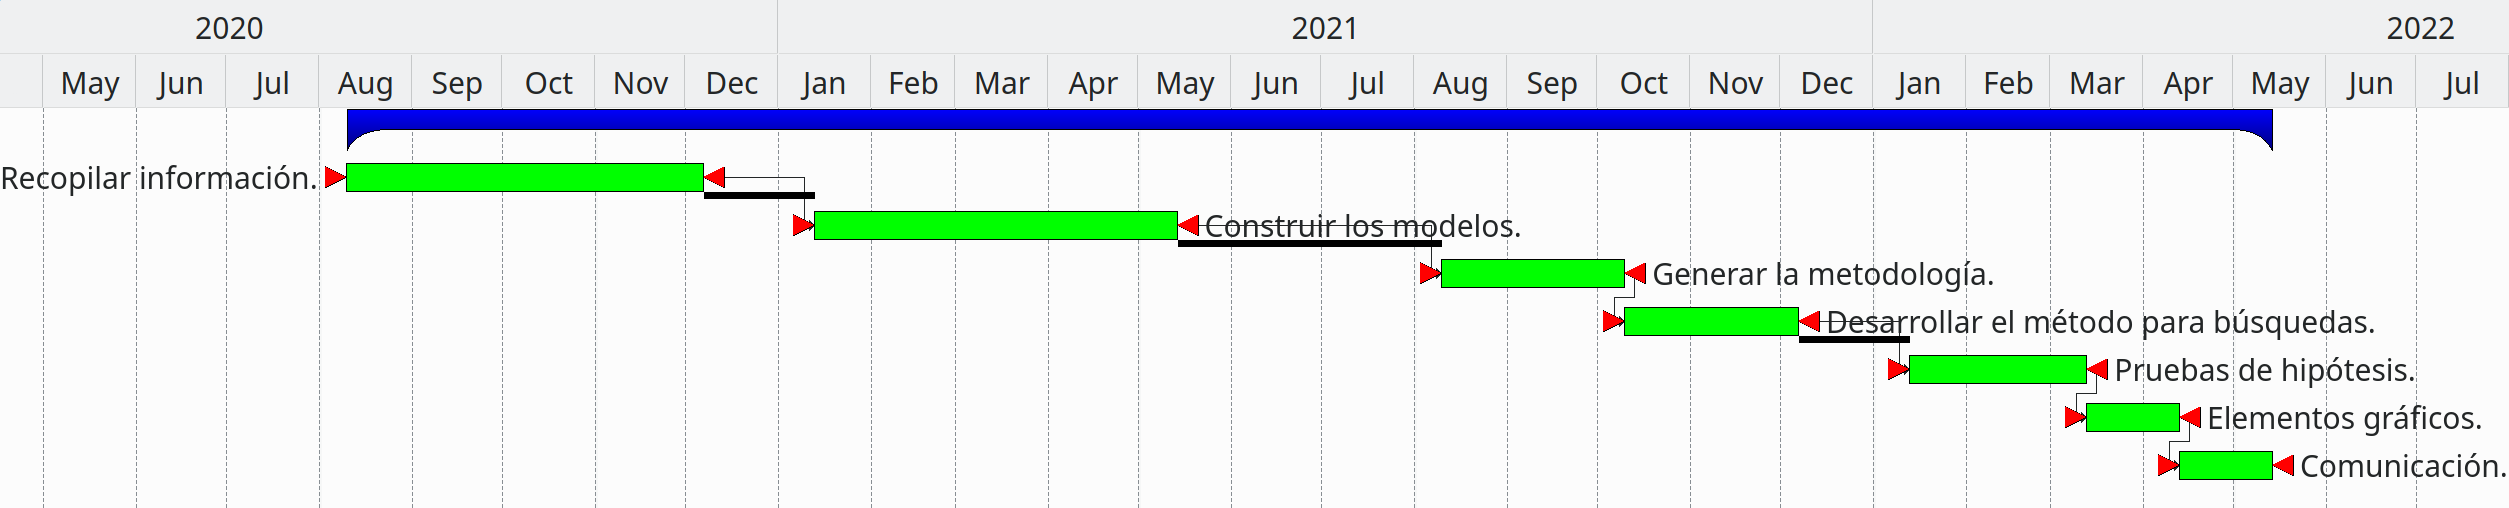
\includegraphics[width=1\linewidth]{gantt.png}\end{figure}